\documentclass[../main.tex]{subfiles}

\graphicspath{{\subfix{../img/}}}

\newcommand{\spazio}{\vspace{1em} \newline}

\begin{document}
    \part{Logica Proposizionale}
    \chapter{La logica}
    \section{Intuizioni iniziali}
    Le caratteristiche della logica proposizionale sono:
    \begin{itemize}
        \item Un linguaggio proposizionale contiene solo proposizioni primitive.
        \item Le formule sono interpretate attraverso un dominio di giudizi.
        \item Le formule complesse sono formate usando un numero arbitrario di connettivi proposizionali.
        \item I connettivi proposizionali possono essere.
        \begin{itemize}
            \item $\lnot$ letto come "not" per la negazione.
            \item $\land$ letto come "and" per le congiunzioni.
            \item $\lor$ letto come "or" per le disgiunzioni.
            \item $\Longrightarrow$ letto come "implies" per le implicazioni.
            \item $\Longleftrightarrow$ letto come "if and only if" per le equivalenze.
            \item $\uparrow$ letto come "nand" per le congiunzioni negate.
            \item $\downarrow$ letto come "nor" per le disngiunzioni negate.
        \end{itemize} 
    \end{itemize}
    La logica proposizionale è utile per problemi che possono essere formalizzati per essere indipendenti da strutture interne.\\
    Sulla logica proposizionale possiamo fare le seguenti osservazioni:
    \begin{itemize}
        \item Una proposizione è una frase che descrive il mondo.
        \item Una proposizione può essere o vera o falsa.
        \item "not P" è vera se P è falsa e viceversa.
        \item "P and Q" è vera se e solo se P e Q sono entrambe vere.
        \item "P or Q" per essere vera è sufficiente che solo una delle due sia vera.
        \item "P implies Q" indica che Q è vera quando lo è P, ma non dice nulla su quando P è falsa.
        \item "P if and only if Q" indica che P e Q devo essere vere/false allo stesso momento.
        \item "P xor Q" è vera solo se una delle due è vera.
    \end{itemize}

    \section{Sintassi}
    \subsection{Alfabeto proposizionale}
    L'alfabeto è composto da:
    \begin{itemize}
        \item Simboli logici: $\lnot, \land, \lor,\supset , \equiv$.
        \item Simboli non logici: costanti proposizionali e insiemi \textbf{PROP} che contengono simboli P chiamati variabili proposizionali che possono contenere una costante proposizionale come un valore.
        \item Simboli separatori: "(" e ")".
    \end{itemize}

    \subsection{Formule ben formate(wff)}
    Una formula wff viene definita come segue:
    \begin{itemize}
        \item Ogni P$\in$\textbf{PROP} è una formula atomica.
        \item Ogni formula atomica è wff.
        \item Se A e B sono formule, allora $\lnot$A, A$\land$B, A$\lor$B, A$\supset$B e A$\equiv$B sono formule.
    \end{itemize}
    Per leggere una formula è importante sapere che i vari operatori hanno delle diverse priorità, come in matematica le parentesi fungono da modificatore delle priorità.
    \begin{center}
        \begin{tabular}{c|c}
            \textbf{Simbolo} & \textbf{Priorità}\\
            \hline
            $\lnot$ & 1\\
            $\land$ & 2\\
            $\lor$ & 3\\
            $\supset$ & 4\\
            $\equiv$ & 5\\
        \end{tabular}
    \end{center}

    \subsection{Sottoformule}
    Una sottoformula di una formula, rappresentata come un albero, indica l'insieme di tutti i suoi sottoalberi.\\
    Viene formalmente definita come:
    \begin{itemize}
        \item A è una sottoformula di se stessa.
        \item A e B sono sottoformule di A$\land$B, A$\lor$B, A$\supset$B e A$\equiv$B.
        \item A è una sottoformula di $\lnot$A.
        \item Se A è una sottoformula di B e B è una sottoformula di C, allora A è una sottoformula di C.
        \item A è una sottoformula propria di B se A è sottoformula di B e A$\neq$B.
    \end{itemize}

    \subsubsection{Esempi}
    \begin{enumerate}
        \item Se piove mentre splende il sole apparirà l'arcobaleno.\\
            p=piove; q=splende il sole; r=arcobaleno;\\
            (p$\land$q)$\supset$r
        \item Claudio viene se Elsa viene.\\
            p=Claudio viene; q=Elsa viene;\\
            q$\supset$p
        \item Claudio viene se Elsa viene e viceversa.\\
            p=Claudio viene; q=Elsa viene;\\
            q$\equiv$p
        \item Giacomo viene se e solo se Pietro resta a casa.\\
            p=Giacomo viene; q=Pietro sta a casa;\\
            p$\equiv$q
        \item Noi andiamo se non piove.\\
            p=Noi andiamo; q=piove;\\
            p$\equiv \lnot$q
        \item Claudio ed Elsa sono o fratello e sorella o nipoti.\\
            p=Claudio ed Elsa sono fratello e sorella; q= Claudio ed Elsa sono nipoti;\\
            p$\lor$q
        \item Se perdo se non posso fare una mossa, allora ho perso.\\
            p=ho perso; q=non posso fare una mossa;\\
            (q$\supset$p)$\supset$p
    \end{enumerate}

    \section{Funzione di interpretazione}
    Il dominio di interpretazione della logica proposizionale è D=\{True, False\}.\\
    L'interpretazione proposizionale è una funzione:
    \begin{center}
        I: \textbf{PROP} $\to$ D
    \end{center}
    Se $|$\textbf{PROP}$|$ è la cardinalità di \textbf{PROP} allora esistono $2^{|\textbf{PROP}|}$ interpretazioni differenti corrispondenti a tutti i sottoinsiemi di \textbf{PROP}.

    \section{Implicazione}
    Diciamo che una funzione di interpretazione implica una formula A se:
    \begin{itemize}
        \item I$\models$A, se I(A)=True con A$\in$\textbf{PROP}.
        \item I$\models \lnot$A, se non è vero che I$\models$A.
        \item I$\models$A$\land$B se I$\models$A e I$\models$B.
        \item I$\models$A$\lor$B se I$\models$A o I$\models$B.
        \item I$\models$A$\supset$B se I$\models$A allora I$\models$B.
        \item I$\models$A$\equiv$B se I$\models$A se e solo se I$\models$B.
    \end{itemize}
    \begin{minipage}{0.5\textwidth}
        \begin{tabular}{|c|c|}
            \hline
            $\lnot$True & False\\
            $\lnot$False & True\\
            \hline
            True $\land$ True & True\\
            True $\land$ False & False\\
            False $\land$ True & False\\
            False $\land$ False & False\\
            \hline
            True $\lor$ True & True\\
            True $\lor$ False & True\\
            False $\lor$ True & True\\
            False $\lor$ False & False\\
            \hline
        \end{tabular}
    \end{minipage}
    \begin{minipage}{0.5\textwidth}
        \begin{tabular}{|c|c|}
            \hline
            True $\supset$ True & True\\
            True $\supset$ False & False\\
            False $\supset$ True & True\\
            False $\supset$ False & True\\
            \hline
            True $\equiv$ True & True\\
            True $\equiv$ False & False\\
            False $\equiv$ True & False\\
            False $\equiv$ False & True\\
            \hline
        \end{tabular}
    \end{minipage}

    \section{Errori comuni}
    \begin{itemize}
        \item Noi esprimiamo le congiunzioni con molte parole oltre a "e", degli esempio posso essere "ma", "quindi ", "per tanto", \dots
        \item Alcune vole "e" non unisce due proposizioni intere ma solo due sostantivi.
        \item Alcune volte "and" unisce due aggettivi.
        \item Il modo per esprimere una disgiunzione esclusiva è (p$\lor$q)$\land \lnot$(p$\lor$q), mentre il modo per indicare che hanno valori di verità diversi è negare la loro uguaglianza $\lnot$(p$\equiv$q).
        \item \textbf{Anche se:} la frase "p anche se q" può essere tradotta in p$\land$(q$\lor \lnot$q).
    \end{itemize}

    \chapter{Calcolo}
    \section{Tabelle di verità}
    Sono il mezzo attraverso il quale generiamo tutte le possibili interpretazioni generate considerando tutte le proposioni atomiche per rispondere ai quesiti di:
    \begin{itemize}
        \item Verifica del modello.
        \item Soddisfabilità.
        \item Validità.
        \item Insoddisfabilità.
        \item Conseguenza logica.
        \item Equivalenza logica.
    \end{itemize}
    Per costruire una tabella di verità, con $n$ proposioni aomiche, è possibile seguire l'algoritmo:
    \begin{enumerate}
        \item Esiste una riga per ogni interpretazione, quindi ne avrò $2^n$.
        \item Le prime $n$ colonne comprendono tutte le interpretazioni, mentre l'ultima i valori di verità della formula totale.\\
            Le colonne nel mezzo contengono i valori di verità delle sottoformule della formula finale presa in considerazione.
        \item L'asseganemnto dei valori alle proposizioni atomiche inizia da sinistra verso destra, nella prima colonnna alterno T e F con periodo 1, nella seconda con periodo 2 e nella $n$ con periodo $n$.
    \end{enumerate}

    \section{Verifica del modello}
    Sia / un interpretazione applicata ad un linguaggio proposizionale L.\\
    Possiamo verificare che una formula A$\in$L è soddisfabile da / applicando in modo ricorsivo l'algoritmo \textbf{MCHECK(I,A)}.

    \subsection{Algoritmo}
    \subsubsection{Caso base}
    A=p
    \begin{lstlisting}
        MCHECK(I$\models$p)
        if I(p)==True then
            return YES
        else
            return NO
    \end{lstlisting}

    \subsubsection{Caso ricorsivo}
    A=B$\land$C
    \begin{lstlisting}
        MCHECK(I$\models$B$\land$C)
        if MCHECK(I$\models$B) then
            return MCHECK(I$\models$C)
        else
            return NO
    \end{lstlisting}

    \noindent
    A=B$\lor$C
    \begin{lstlisting}
        MCHECK(I$\models$B$\lor$C)
        if MCHECK(I$\models$B) then
            return YES
        else
            return MCHECK(I$\models$C)
    \end{lstlisting}

    \noindent
    A=B$\supset$C
    \begin{lstlisting}
        MCHECK(I$\models$B$\supset$C)
        if MCHECK(I$\models$B) then
            return MCHECK(I$\models$C)
        else
            return YES
    \end{lstlisting}

    \noindent
    A=B$\equiv$C
    \begin{lstlisting}
        MCHECK(I$\models$B$\equiv$C)
        if MCHECK(I$\models$B) then
            return MCHECK(I$\models$C)
        else
            return $\lnot$MCHECK(I$\models$C)
    \end{lstlisting}

    \section{Soddisfacibilità}
    Possiamo controllare che qualsiasi formula A$\in$L è soddisfabile applicando l'algoritmo \textbf{SAT(A)} che è definito come segue:
    \begin{itemize}
        \item \textbf{Input:} inseriamo la formula A della quale vogliamo sapere se esiste un interpretazione che la soddisfa.
        \item \textbf{Output:} ci viene restituita l'interpretazione se la formula è soddisfabile in caso contrario viene ritornato "no".
        \item Possiamo verificare A sia soddisfabile applicando in moso ricorsivo \textbf{MCHECK(I,A)} come segue:
        \begin{itemize}
            \item Estrarre tutte le proposizioni atomiche di A.
            \item Generare tutte le interpretazioni I utili.
            \item Applicare \textbf{MCHECK(I,A)} finchè non si verifica una delle due condizioni.
        \end{itemize}
        \begin{enumerate}
            \item Se \textbf{MCHECK(I,A)} ritorna "YES" allora viene ritornato I.
            \item Se non ci sono più I da analizare viene ritornato "NO".
        \end{enumerate}
        \item \textbf{SAT(A)} compie una cosidetta lazy evaluation infatti salta le interpretazioni quando irrilevanti così evita di valutare $2^n$ casi.
    \end{itemize}

    \subsubsection{Esempio}
    Controllo se (P$\land$Q)$\lor$(R$\supset$S) è soddisfabile.\\
    Devo calcolare tutte le possibile I:
    \begin{itemize}
        \item \{P, Q, R, S\}
        \item \{P, Q, R\}
        \item \{P, Q\}\\
        \vdots
    \end{itemize}
    Per ogni I rimpiazzare i valori di verità corrispondenti nelle primitive.\\
    Con I=\{P\} abbiamo che:
    \begin{center}
        (True$\land$False)$\lor$(False$\supset$False)\\
        False$\lor$True\\
        True
    \end{center}
    Quindi la formula è soddisfabile.

    \section{Validità}
    Possiamo controllare che qualsiasi formula A$\in$L sia valida applicando l' algoritmo \textbf{VALID(A)} come segue.
    \begin{itemize}
        \item \textbf{Input:} inseriamo la formula A della quale vogliamo sapere se è soddisfabile per ogni interpretazione.
        \item \textbf{Output:} viene ritornato "YES" se è una formula valida, "NO" altrimenti.
        \item Possiamo ora verificare che A sia valida applicando \textbf{MCHECK(I,A)} come segue:
        \begin{itemize}
            \item Estrarre tutte le proposizioni atomiche di A.
            \item Generare tutte le interpretazioni I utili.
            \item Applicare \textbf{MCHECK(I,A)} finchè non si verifica una delle due condizioni.
        \end{itemize}
        \begin{enumerate}
            \item Se un \textbf{MCHECK(I,A)} ritorna "NO" allora tutta la funzione ritorna "NO".
            \item Se non ci sono più formule da analizzare ritorna "YES".
        \end{enumerate}
        \item \textbf{VALID(A)} compie  una lazy evaluation così appena una parte ritorna "NO" si ferma.
    \end{itemize}

    \subsubsection{Esempio}
    Controllo se (P$\land$Q)$\lor$(R$\supset$S) è valida.\\
    Devo calcolare tutte le possibile I:
    \begin{itemize}
        \item \{P, Q, R, S\}
        \item \{P, Q, R\}
        \item \{P, Q\}\\
        \vdots
    \end{itemize}
    Per ogni I rimpiazzare i valori di verità corrispondenti nelle primitive.\\
    Con I=\{P, R\} abbiamo che:
    \begin{center}
        (True$\land$False)$\lor$(True$\supset$False)\\
        False$\lor$False\\
        False
    \end{center}
    Essendo un interpretazione falsa la formula non è valida.

    \section{Insoddisfabilità}
    Possiamo dire per una qualsiasi formula A$\in$L se è insoddisfabile applicando l'algoritmo \textbf{UNSAT(A)} come segue:
    \begin{itemize}
        \item \textbf{Input:} inseriamo la formula A della quale vogliamo sapere se è insoddisfabile.
        \item \textbf{Output:} ritorna "YES" se nessuna I soddisfa A, ritorna "NO" altrimenti.
        \item Possiamo ora verificare che A sia insoddisfabile applicando \textbf{MCHECK(I,A)} come segue:
        \begin{itemize}
            \item Estrarre tutte le proposizioni atomiche di A.
            \item Generare tutte le interpretazioni I utili.
            \item Applicare \textbf{MCHECK(I,A)} finchè non si verifica una delle due condizioni.
        \end{itemize}
        \begin{enumerate}
            \item Se un \textbf{MCHECK(I,A)} ritorna "YES" allora si ritorna "NO".
            \item Se non ci sono più formule da analizzare ritorna "YES".
        \end{enumerate}
    \end{itemize}

    \subsubsection{Esempio}
    Controllo se (P$\land$Q)$\lor$(R$\supset$S) è invalida.\\
    Calcolo tutti i possibili I.\\
    Prendo I=\{P\} abbiamo che:
    \begin{center}
        (True$\land$False)$\lor$(False$\supset$False)\\
        False$\lor$True\\
        True
    \end{center}
    In questo caso \textbf{UNSAT(A)} ritornerà "NO" perchè la formula è soddisfabile.

    \section{Correlazioni tra validità soddisfacibilità e insoddisfabilità}
    Queste 3 proprietà sono legate tra di loro.\\
    \textbf{Proposizione 1:} se una formula è valida allora è soddisfabile e anche non insoddisfabile.
    \begin{center}
        valida$\supset$soddisfabile$\supset \lnot$insoddisfabile
    \end{center}
    \textbf{Proposizione 2:} se una formula è insoddisfabile allora è non soddisfabile e non valida.
    \begin{center}
        insoddisfabile$\supset \lnot$soddisfabile$\supset \lnot$valida
    \end{center}
    \textbf{Proposzione 3:} data una formula A allora vale che:
    \begin{center}
        \begin{tabular}{c c}
            \hline
            A & $\lnot$A\\
            \hline
            \hline
            valida & insoddisfabile\\
            soddisfabile & $\lnot$valida\\
            $\lnot$valida & soddisfabile\\
            insoddisfabile & valida\\
        \end{tabular}
    \end{center}
    \textbf{Proposizione 4:}Per un qualsiasi insieme finito $\Gamma$ di formule($\text{A}_1$, \dots $\text{A}_n$ con $n\ge1$) possiamo dire che $\Gamma$ è:
    \begin{itemize}
        \item Valido se e solo se $\text{A}_1 \land \dots \land \text{A}_n$ è valida.
        \item Soddisfabile se e solo se $\text{A}_1 \lor \dots \lor \text{A}_n$ è soddisfabile.
        \item Insoddisfabile se e solo se $\text{A}_1 \lor \dots \lor \text{A}_n$ è insoddisfabile
    \end{itemize}

    \section{Conseguenza logica}
    Possiamo capire se una qualsiasi $\text{T}_1 \models \text{T}_2$ è valida applicando l'algoritmo \textbf{LOGCONS($\text{T}_1$,$\text{T}_2$)} come segue:
    \begin{itemize}
        \item \textbf{Input:} T$_1$ è la teoria di partenza che assumo esssere vera mentre T$_2$ è quella che deve seguire o meno T$_1$.
        \item \textbf{Output:} ritorna "YES" se T$_2$ segue da T$_1$, "NO" altrimenti.
        \item Possiamo ora verificare che sia una conseguenza logica come segue:
        \begin{itemize}
            \item Genero tutte le interpretazioni utili I.
            \item Applico sistematicamente \textbf{MCHECK(I,T$_1$)} con i seguenti risultati:
        \end{itemize}
        \begin{enumerate}
            \item Se \textbf{MCHECK(I,T$_1$)} ritorna "YES" applico \textbf{MCHECK(I,T$_2$)} che se ritoena "NO" faccio ritornare "NO" da tutto.
            \item Se non ci sono più I da analizzare ritorno "YES".
        \end{enumerate}
    \item \textbf{LOGCONS($\text{T}_1$,$\text{T}_2$)} compie una lazy evaluation quando una chiamata ritorna "NO".
    \end{itemize}

    \section{Equivalenza logica}
    Possiamo capire se una qualsiasi $\text{T}_1$ e $\text{T}_2$ sono logicamente equivalenti con l'algoritmo \textbf{LOGEQ($\text{T}_1$,$\text{T}_2$)} come segue:
    \begin{itemize}
        \item \textbf{Input:} T$_1$ è la teoria di partenza che assumo esssere vera mentre T$_2$ è quella che deve essere equivalente o meno T$_1$.
        \item \textbf{output:} ritorna "YES se sono equivalenza logica, "NO" altrimenti.
        \item Possiamo verificare che due teorie sono un'equivalenza logica applicando l'algoritmo:
        \begin{itemize}
            \item Genero le interpretazioni che potrebbero essermi utili.
            \item Applico \textbf{MCHECK(I,T$_1$)} e  \textbf{MCHECK(I,T$_2$)}.
            \item Se i risultati sono diversi ritorno "NO", ritorno "YES" altrimenti.
        \end{itemize}
    \end{itemize}

    \chapter{La procedura di decisione DPLL}
    \section{Nozioni di base}
    SAT o UNSAT sono delle proprietà chiave che indicano se una teoria può essere applicata in pratica.\\
    PL SAT è un prblema NP-completo quindi tutti i problemi NP-completi posso essere codificati in SAT.\\
    \textbf{Teorema di deduzione:} data $\Gamma$, se $\phi \models \psi$ allora $\Gamma \models \phi \supset \psi$ con $\Gamma$ possibilmente vuota.

    Questo ci permette di ridurre il problema dalla verifica della conseguenza logica ad PL SAT.\\
    PL SAT può essere ridotto con l'uso di CNF PL SAT(Conjunctive Normal Form), a questo punto CNF SAT può essere risolto in modo molto efficente usando l'euristica.

    \section{CNF(Conjunctive Normal Form)}
    Definizioni:
    \begin{itemize}
        \item \textbf{Letterale:} è o una variabile proposizionale oppure il negato di una variabile proposizionale, due esempi sono le formule $p$ e $\lnot p$.
        \item \textbf{Clausole:} è una disgiunzione($\lor$) di letterali.
        \item \textbf{CNF(Conjunctive Normal Form):} una formula è in CNF se è una congiunzione di varie clausole per esempio: 
            \begin{center}
                $(p \lor \lnot q \lor r) \land (q \lor r) \land (\lnot p \lor \lnot q) \land r$ 
            \end{center}
            Una CNF ha sempre la seguente formula:
            \begin{center}
                $(L_{(1,1)} \lor \dots \lor L_{(1,n_1)})\land \dots \land (L_{(m,1)} \lor \dots \lor L_{(m,n_m)})$
            \end{center}
            Scritto anche come:
            \begin{center}
                $\bigwedge^{m}_{i=1} (\bigvee^{n_j}_{j=1} L_{i,j})$
            \end{center}
            dove $L_{i,j}$ è il j-esimo letterale della i-esima formula.
    \end{itemize}
    Proprietà delle clausole:
    \begin{itemize}
        \item L'ordine dei letterali in una clausola non importa $\phi \lor \psi \equiv \psi \lor \phi$, infatti $(p \lor q \lor r \lor \lnot r ) \equiv (\lnot r \lor q \lor p \lor r)$.
        \item Alcuni letterali possono essere uniti, se una clausola c'è più di un'occorrenza dil un letterale posso spostare i due uguali vicini per unirli $\phi \lor \phi \equiv \phi$, infatti $(p \lor q \lor r \lor q \lor \lnot r ) \equiv (p \lor q \lor r \lor \lnot r )$.
        \item Le clausole sono insiemi di letterali, possiamo costruire un insieme togliendo le disgiunzioni e ignorano le ripetizioni, infatti $(p \lor q \lor r \lor \lnot r)$ è rappresentato da $\{p, q, r, \lnot r\}$.
    \end{itemize}
    Proprietà delle formule CNF:
    \begin{itemize}
        \item L'ordine delle clausole non importa se una formula CNF $\phi$ è ottenuta riordinando i termini di una formula CNF $\phi \prime$ allora $\phi \equiv \phi \prime$.
        \item Le clausole uguali posso essere unite in una unica clausola.
        \item Una formula in CNF può essere vista come un insieme clausole.
        \item \textbf{Esistenza:} ogni formula può essere riscritta in CNF.
        \item \textbf{Equivalenza:} $\models$ CNF($\phi$)$\equiv \phi$.
        \item \textbf{Funzione CNF:} data una formula PL $\phi$ la funzione CNF(\dots) che trasforma $\phi$ nella sua forma CNF è definita ricorsivamente:
            \begin{align*}
                CNF(p)&=\text{p se p} \in \textbf{PROP}\\
                CNF(\lnot p) &=\text{$\lnot$p se p} \in \textbf{PROP}\\
                CNF(\phi \supset \psi) &= CNF(\lnot \phi) \otimes CNF(\psi)\\
                CNF(\phi \land \psi) &= CNF(\phi) \land CNF(\psi)\\
                CNF(\phi \lor \psi) &= CNF(\phi) \otimes CNF(\psi)\\
                CNF(\phi \equiv \psi) &= CNF(\phi \supset \psi) \land CNF(\psi \supset \phi)\\
                CNF(\lnot \lnot \phi) &= CNF(\phi)\\
                CNF(\lnot (\phi \supset \psi)) &= CNF(\phi) \land CNF(\lnot \psi)\\
                CNF(\lnot (\phi \land \psi)) &= CNF(\lnot \phi) \otimes CNF(\lnot \psi)\\
                CNF(\lnot (\phi \lor \psi)) &= CNF(\lnot \phi) \land CNF(\lnot \psi)\\
                CNF(\lnot (\phi \equiv \psi)) &= CNF(\phi \land \lnot \psi) \otimes CNF(\psi \land \lnot \phi)
            \end{align*}
            Dove $(C_1 \land \dots \land C_n) \otimes (D_1 \land \dots \land D_m)$ è definito come:
            \begin{center}
                $(C_1 \lor D_1) \land \dots \land(C_1 \lor D_m) \land \dots \land(C_n \lor D_1) \land \dots \land(C_n \lor D_m)$
            \end{center}
    \end{itemize}

    \subsubsection{Esempio di CNF}
    Proviamo ora a trasformare in CNF la seguente formula:
    \begin{gather*}
        p1 \equiv (p2 \equiv (p3 \equiv (p4 \equiv (p5 \equiv p6)))) \\
        CNF(p1 \supset (p2 \equiv (p3 \equiv (p4 \equiv (p5 \equiv p6))))) \land CNF((p2 \equiv (p3 \equiv (p4(p5 \equiv p6)))) \supset p1)\\
        \vdots
    \end{gather*}
    la lunghezza della formula diventa di lunghezza esponenziale se si continua, nel caso peggiore la formula CNF($\phi$) è esponenzialmente lunga rispetto a $\phi$ però calcolare la validità/insoddisfabilità di una formula CNF richiede un tempo lineare.

    \section{Soddisfabilità di una formula in CNF}
    Sia $CNF(\phi)=C_0, \dots ,C_n$ dove $C_0,\dots ,C_n$ sono le clausola in CNF($\phi$), allora vale che:
    \begin{itemize}
        \item $I \models \phi$ se e solo se $I \models C_i$ per ogni i=0, \dots, n.
        \item $I \models C_i$ se e solo se per un letterale $k \in C_i$, $I \models k$.
    \end{itemize}
    Per vedere se un modello $I$ soddisfa $N$ non abbiamo bisogno di conoscere tutti i valori dei letterali che appaiono in $N$.\\
    Per esempio se $I(P)$=True e $I(q)$=false possiamo dire che $I \models \{\{p, q, \lnot r\}, \{\lnot q, s\}\}$.\\
    Possiamo usare una funzione parziale per assegnare ad alcune variabili dell' alfabeto il valore di verità, grazie a questa valutazione parziale possimo dire che i letterali o le clausole sono True, False o Undefined.
    \begin{itemize}
        \item \textbf{True:} una clausola è True se secondo $I$ almeno uno dei suoi ltterali è True.
        \item \textbf{False:} una clausola è falsa se tutti i suoi letterali sono falsi.
        \item \textbf{Undefined:} quando il valore di verità dei suoi letterali è irrilevante per l'interpretazione corrente.
    \end{itemize}
    \textbf{Semplificazione di formule attraverso letterali positivi:} per una formula in CNF $\phi$ ed il termine $p$ allora $\phi |_p$ indica la formula ottenuta da $\phi$ con:
    \begin{itemize}
        \item Rimpiazzando tutte le occorrenze di $p$ con il valore $\top$.
        \item Semplificando il risultato rimuovendo:
        \begin{itemize}
            \item Le clausole contenenti il termine disgiuntivo $\top$.
            \item I letterali $\lnot \top = \perp$ nelle formule rimanenti.
        \end{itemize}
    \end{itemize}
    \textbf{Semplificazione di formule attraverso letterali negativi:} per una formula in CNF $\phi$ ed il termine $p$ allora $\phi |_{\lnot p}$ indica la formula ottenuta da $\phi$ con:
    \begin{itemize}
        \item Rimpiazzando tutte le occorrenze di $\lnot p$ con il valore $\perp$.
        \item Semplificando il risultato rimuovendo:
        \begin{itemize}
            \item Le clausole contenenti i termini di disgiunzione $\lnot \top = \perp$.
            \item I letterali $\top$ nelle clausole rimanenti.
        \end{itemize}
    \end{itemize}
    \textbf{Soddisfabilità di una CNF:} sia una $CNF(\phi)=C_0 \dots C_n$ dove i termini sono le clausole delle formula, iteriamo il processo di valutazione letterale, alla fine possiamo finire con due alternative:
    \begin{enumerate}
        \item \{\}, cioè un insieme vuoto di clausole quindi $\phi$ è soddisfabile.
        \item \{\dots \{\} \dots \} se sono riuscito a semplificare solo parte delle clausole vuol dire che $\phi$ è insoddisfabile.
    \end{enumerate}

    \subsubsection{Esempio}
    \begin{equation*}
        (p \lor q) \land (p \lor \lnot p) \land (\lnot q \lor q) \land (\lnot q \lor \lnot p) \land (\lnot q \lor \lnot p) \land (\lnot q \lor \lnot p) \land ( \lnot q \lor q )\land (p \lor \lnot p) \land (p \lor q)
    \end{equation*}
    Prima cosa faccio il merge delle clausole uguali:
    \begin{equation*}
        (p \lor q) \land (p \lor \lnot p) \land (\lnot q \lor q) \land (\lnot q \lor \lnot p) 
    \end{equation*}
    Ora divido in insiemi:
    \begin{equation*}
        \{ \{p,q\}, \{p,\lnot p\}, \{\lnot q,q\}, \{\lnot q,\lnot p\} \}
    \end{equation*}
    Posso ora applicare una semplificazione per termini positivi in $p$ quindi $\phi|_p$
    \begin{equation*}
        \{ \{\top,q\}, \{ \top , \perp \}, \{\lnot q,q\}, \{\lnot q,\perp \} \}
    \end{equation*}
    Rimango quindi con:
    \begin{equation*}
        \{ \{q\}, \{\lnot q,q\}, \{\lnot q \} \}
    \end{equation*}
    Semplifico ora in $\lnot q$ quindi $\phi|_{\lnot q}$
    \begin{equation*}
        \{ \{ \perp \}, \{\top , \perp \}, \{\top \} \}
    \end{equation*}
    Semplificando rimango con \{\} quindi la formula è soddisfabile.

    \section{La procedura di decisione}
    \subsection{Semplificazione con unità di propagazione}
    \textbf{Clausola unita:} se una formula in CNF $\phi$ contiene una clausola $C=\{I\}$ che consiste un singolo letterale $I$ nel suo insieme.
    \subsubsection{Esempio}
    Prendiamo la formula in CNF $\phi=\{\{p\}, \{\lnot p\}, \{\lnot q, r \}\}$ è soddisfabile solo se se esiste un'interpretazione $I$ tale che $I \models \phi$.
    \begin{gather*}
        \{\{p\}, \{\lnot p\}, \{\lnot q, r \}\}|_p\\
        \{\{ \top \}, \{ \perp \}, \{\lnot q, r \}\}\\
        \{\{\}, \{\lnot q, r \} \}\\
        \{ \dots,\{\}, \dots\}
    \end{gather*}
    Quindi la formula non è soddisfabile.
    
    \subsubsection{Osservazioni}
    \begin{itemize}
        \item Ci sono casi in cui l'unità di propagazione non genera una delle condizioni di terminazione, quindi dobbiamo asseganre noi "a occhio" i valori di verità ai letterali.
        \item Ogni letterale genererà un ramo per ogni valore di verità, da qui nasce la quantità esponenziale di funzioni da analizzare.
    \end{itemize}

    \subsubsection{Algoritmo DPLL}
    \begin{lstlisting}
        DPLL($\phi$, I)
        if $\phi$ contains the empty clause {} then
            return False;
        end
        if $\phi$ = {} then
            exit with I;
        end
        select a literal I $\in$ C $\in$ $\phi$
        DPLL($\phi |$k , I $\cup$ (I(k) = true)) or DPLL($\phi | \lnot$k , I $\cup$ (I(k) = true))
    \end{lstlisting}
    Per arrivare ad una soglia di efficenza c'è bisogno di fare delle scelte euristiche che se si rivelano sbagliate vanno corrette con backtrack.
    \subsubsection{Esempio}
    Considerando la formula $(p \lor \lnot q) \land (p \lor r) \land (\lnot p)$ dobbiamo allora creare l'albero:
    \begin{center}
        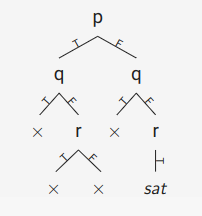
\includegraphics[width=4.5cm,height=4cm,angle=0]{../img/albero_DPLL.png}
    \end{center}

    \subsection{Algoritmo DPLL con unità di propagazione}
    \begin{lstlisting}
        Input: un insieme di clausole $\phi$.
        Output: Una tabella di verita' che indica quando $\phi$ e' soddisfabile.

        function DPLL($\phi$)
            while esiste una clausola {l} in $\phi$ do
                $\phi$ $\leftarrow$ unit-propagate(l, $\phi$);
            while esiste un letterale L che appare in $\phi$ do
                $\phi$ $\leftarrow$ pure-literal-assign(l, $\phi$);
            if $\phi$ is empty then return true;
            if $\phi$ contains an empty clause then return false;
            l $\leftarrow$ select-literal($\phi$);
            DPLL($\phi$ $\land$ {l}) or DPLL($\phi$ $\land$ {$\lnot$ (l)});
    \end{lstlisting}

    \chapter{Decisione procedura basata su Tableau}
    \section{Nozioni di base}
    Dobbiamo capire perchè i Tableau possono risolvere il problema di SAT.\\
    \textbf{Principio di confutazione:} ci permette di trasformare un problema di conseguenza logica in uno di insoddisfabilità.
    \begin{center}
        $\Gamma \models \phi$ se e solo se $\Gamma \cup \{ \lnot \phi \}$
    \end{center}
    Come con DPLL vengono dati input all'algoritmo solo le formule rilevanti per la valutazione.\\
    Anche se con i Tableau non serve che la formula sia in CNF e il passo di inferenza è diverso da DPLL anche se creano un algoritmo per la nozione di implicazione.\\
    I Tableau sono, infatti, una rappresentazione diretta della definizione di implicazione questo lo rende concettualmente più semplice da capire ma anche più difficile da scalare su formule complesse.

    \section{Sistema Tableau}
    \textbf{Tableau:} il metodo basato su Tableau è composto da 3 elementi:
    \begin{enumerate}
        \item Un insieme di premesse $\Gamma$ e di conclusioni $\phi$.
        \item Un compito, provare che $\Gamma \models \phi$.
        \item Le procedure che dimostrano che $\Gamma \cup \{\lnot \phi\}$ non è soddisfabile, oppure che $\Gamma \cup \{\phi\}$ è valido quindi soddisfabile
    \end{enumerate}
    \textbf{Tableau proposizionali:} è un albero con radice dove:
    \begin{itemize}
        \item Ogni nodo indica una proposizione.
        \item La radice è la formula che dobbiamo provare insoddisfabile.
        \item I fogli di un nodo $n$ sono generati con apposite regole di espansione ad $n$ o ad uno dei suoi antenati.
    \end{itemize}

    \subsection{Regole $\alpha$}
    \begin{minipage}{0.333333\textwidth}
        \begin{gather*}
            \phi \land \psi\\
            \downarrow\\
            \phi\\
            \psi
        \end{gather*}
    \end{minipage}
    \begin{minipage}{0.333333\textwidth}
        \begin{gather*}
            \lnot (\phi \lor \psi)\\
            \downarrow\\
            \lnot \phi\\
            \lnot \psi
        \end{gather*}
    \end{minipage}
    \begin{minipage}{0.333333\textwidth}
        \begin{gather*}
            \lnot (\phi \supset \psi)\\
            \downarrow\\
            \phi\\
            \lnot \psi
        \end{gather*}
    \end{minipage}
    Le regole $\alpha$ sono congiuntive quindi creano un solo figlio.

    \subsubsection{Esempio}
    \begin{gather*}
        \lnot (p \supset (q \lor \lnot (p \land r )))\\
        \downarrow\\
        p\\
        \lnot (q \lor \lnot (p \land r ))\\
        \downarrow\\
        \lnot q\\
        p \land r\\
        \downarrow\\
        p\\
        r 
    \end{gather*}

    \subsection{Regole $\beta$}
    \begin{center}
        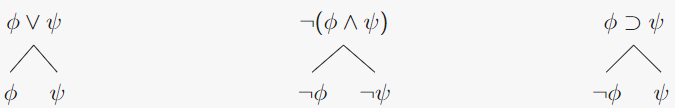
\includegraphics{beta_rules.png}
    \end{center}
    Le regole $\beta$ sono disgiuntive quindi creano due rami distinti che sono entrambi da completare, e quindi bene lasciare queste regole per ultime e usarle solo se necessario.

    \subsection{Controllare la soddisfacibilità}
    Se vogliamo controllare che $\Gamma$ sia soddisfabile metto nella radice del Tableau $\Gamma$ e applico le regole, se almeno un ramo non chiude vuol dire che che è soddisfabile e dal quel ramo possiamo prendere i valori da dare ai termini atomici.

    \subsection{Derivazione}
    Siano $\phi$ una formula proposizionale e $\Gamma$ un insieme di formule proposizionali, scriveremo $\Gamma \vdash \phi$ se esiste un Tableau chiuso per $\Gamma \cup \{\lnot \phi\}$.

    \subsection{Utilità}
    \begin{itemize}
        \item Una formula è insoddisfabile se e solo se oddisfabile, per testare che $\phi$ sia valida basta testare che il Tableau chiuda tutti i rami di $\lnot \phi$.
        \item Per verificare che $\phi$ è una conseguenza logica di $\Gamma$ quindi $\Gamma \models \phi$basta verificare con un Tableau che $\Gamma \land \lnot phi$ che un ramo chiuda.
        \item Per verificare l'equivalenza logica basta ricondursi al caso di conseguenza logica.
    \end{itemize}
    Per riassumere:
    \begin{center}
        \begin{tabular}{|c|c|c|}
            \hline
            Formula & Tableau & Significato\\
            \hline
            $p$ & Chiude & $p$ è insoddisfabile, $\lnot p$ è valida\\
            \hline
            $p$ & Aperto & $p$ è soddisfabile\\
            \hline
            $\lnot p$ & Chiude & $\lnot p$ è insoddisfabile, $p$ è valida\\
            \hline
            $\lnot p$ & Aperto & $\lnot p$ è soddisfabile\\
            \hline
        \end{tabular}
    \end{center}

    \subsection{Teoremi finali}
    \begin{itemize}
        \item \textbf{Terminazione:} per ogni Tableau proposizionale dopo un numero finito di espansioni nessuna regola è più applicabile.
        \item \textbf{Equità:} definiamo così un Tableau proposizionale quando ogni non-letterale di un ramo viene analizzato in quel ramo.
        \item \textbf{Solidità:} Se $\Gamma \vdash \phi$ allora $\Gamma \models \phi$.
        \item \textbf{Completezza:} Se $\Gamma \models \phi$ allora $\Gamma \vdash \phi$.
    \end{itemize}
\end{document}